%%%%%%%%%%%%%%%%%%%%%%%%%%%%%%%%%%%%%%%%%
% Journal Article
% LaTeX Template
% Version 1.3 (9/9/13)
%
% This template has been downloaded from:
% http://www.LaTeXTemplates.com
%
% Original author:
% Frits Wenneker (http://www.howtotex.com)
%
% License:
% CC BY-NC-SA 3.0 (http://creativecommons.org/licenses/by-nc-sa/3.0/)
%
%%%%%%%%%%%%%%%%%%%%%%%%%%%%%%%%%%%%%%%%%

%----------------------------------------------------------------------------------------
%  PACKAGES AND OTHER DOCUMENT CONFIGURATIONS
%----------------------------------------------------------------------------------------

\documentclass[twoside]{article}\usepackage[]{graphicx}\usepackage[]{color}
%% maxwidth is the original width if it is less than linewidth
%% otherwise use linewidth (to make sure the graphics do not exceed the margin)
\makeatletter
\def\maxwidth{ %
  \ifdim\Gin@nat@width>\linewidth
    \linewidth
  \else
    \Gin@nat@width
  \fi
}
\makeatother

\definecolor{fgcolor}{rgb}{0.345, 0.345, 0.345}
\newcommand{\hlnum}[1]{\textcolor[rgb]{0.686,0.059,0.569}{#1}}%
\newcommand{\hlstr}[1]{\textcolor[rgb]{0.192,0.494,0.8}{#1}}%
\newcommand{\hlcom}[1]{\textcolor[rgb]{0.678,0.584,0.686}{\textit{#1}}}%
\newcommand{\hlopt}[1]{\textcolor[rgb]{0,0,0}{#1}}%
\newcommand{\hlstd}[1]{\textcolor[rgb]{0.345,0.345,0.345}{#1}}%
\newcommand{\hlkwa}[1]{\textcolor[rgb]{0.161,0.373,0.58}{\textbf{#1}}}%
\newcommand{\hlkwb}[1]{\textcolor[rgb]{0.69,0.353,0.396}{#1}}%
\newcommand{\hlkwc}[1]{\textcolor[rgb]{0.333,0.667,0.333}{#1}}%
\newcommand{\hlkwd}[1]{\textcolor[rgb]{0.737,0.353,0.396}{\textbf{#1}}}%

\usepackage{framed}
\makeatletter
\newenvironment{kframe}{%
 \def\at@end@of@kframe{}%
 \ifinner\ifhmode%
  \def\at@end@of@kframe{\end{minipage}}%
  \begin{minipage}{\columnwidth}%
 \fi\fi%
 \def\FrameCommand##1{\hskip\@totalleftmargin \hskip-\fboxsep
 \colorbox{shadecolor}{##1}\hskip-\fboxsep
     % There is no \\@totalrightmargin, so:
     \hskip-\linewidth \hskip-\@totalleftmargin \hskip\columnwidth}%
 \MakeFramed {\advance\hsize-\width
   \@totalleftmargin\z@ \linewidth\hsize
   \@setminipage}}%
 {\par\unskip\endMakeFramed%
 \at@end@of@kframe}
\makeatother

\definecolor{shadecolor}{rgb}{.97, .97, .97}
\definecolor{messagecolor}{rgb}{0, 0, 0}
\definecolor{warningcolor}{rgb}{1, 0, 1}
\definecolor{errorcolor}{rgb}{1, 0, 0}
\newenvironment{knitrout}{}{} % an empty environment to be redefined in TeX

\usepackage{alltt}

\usepackage{lipsum} % Package to generate dummy text throughout this template

\usepackage[sc]{mathpazo} % Use the Palatino font
%\usepackage[T1]{fontenc} % Use 8-bit encoding that has 256 glyphs
\usepackage[utf8]{inputenc}
\linespread{1.05} % Line spacing - Palatino needs more space between lines
\usepackage{microtype} % Slightly tweak font spacing for aesthetics

\usepackage[hmarginratio=1:1,top=32mm,columnsep=20pt]{geometry} % Document margins
\usepackage{multicol} % Used for the two-column layout of the document
\usepackage[hang, small,labelfont=bf,up,textfont=it,up]{caption} % Custom captions under/above floats in tables or figures
\usepackage{booktabs} % Horizontal rules in tables
\usepackage{float} % Required for tables and figures in the multi-column environment - they need to be placed in specific locations with the [H] (e.g. \begin{table}[H])
\usepackage{hyperref} % For hyperlinks in the PDF

\usepackage{lettrine} % The lettrine is the first enlarged letter at the beginning of the text
\usepackage{paralist} % Used for the compactitem environment which makes bullet points with less space between them

\usepackage{color} % used to mark parts that need to be edited

\usepackage{abstract} % Allows abstract customization
\renewcommand{\abstractnamefont}{\normalfont\bfseries} % Set the "Abstract" text to bold
\renewcommand{\abstracttextfont}{\normalfont\small\itshape} % Set the abstract itself to small italic text

\usepackage{titlesec} % Allows customization of titles
\renewcommand\thesection{\Roman{section}} % Roman numerals for the sections
\renewcommand\thesubsection{\Roman{subsection}} % Roman numerals for subsections
\titleformat{\section}[block]{\large\scshape\centering}{\thesection.}{1em}{} % Change the look of the section titles
\titleformat{\subsection}[block]{\large}{\thesubsection.}{1em}{} % Change the look of the section titles

\usepackage{fancyhdr} % Headers and footers
\pagestyle{fancy} % All pages have headers and footers
\fancyhead{} % Blank out the default header
\fancyfoot{} % Blank out the default footer
\fancyhead[C]{Running title $\bullet$ November 2012 $\bullet$ Vol. XXI, No. 1} % Custom header text
\fancyfoot[RO,LE]{\thepage} % Custom footer text
\bibliographystyle{plain}

%%%-------------------------------------------------%%%
%%% Preferences for Knitr %%%
%%%-------------------------------------------------%%%


%%%-------------------------------------------------%%%
%%% Sub document global preferences for Knitr %%%
%%%-------------------------------------------------%%%










%----------------------------------------------------------------------------------------
%  TITLE SECTION
%----------------------------------------------------------------------------------------

\title{\vspace{-15mm}\fontsize{24pt}{10pt}\selectfont\textbf{Assessing economic inequality with tax data - Switzerland from 1945 to 2010}} % Article title

\author{
\large
\textsc{Oliver Hümbelin}\\[2mm] % Your name
\normalsize Bern University of Applied Sciences \\ % Your institution
\normalsize \href{mailto:oliver.huembelin@bfh.ch}{oliver.huembelin@bfh.ch} % Your email address
\vspace{5mm}\\
\large
\textsc{Rudolf Farys}\\[2mm] % Your name
\normalsize University of Bern \\ % Your institution
\normalsize \href{mailto:rudolf.farys@soz.unibe.ch}{rudolf.farys@soz.unibe.ch} % Your email address
\vspace{-5mm}
}
\date{}

%----------------------------------------------------------------------------------------
\IfFileExists{upquote.sty}{\usepackage{upquote}}{}

\begin{document}

\maketitle 

\thispagestyle{fancy} % All pages have headers and footers

%----------------------------------------------------------------------------------------
%	ABSTRACT
%----------------------------------------------------------------------------------------

%%%-------------------------------------------------%%%
%%% Include abstract %%%
%%%-------------------------------------------------%%%


%%%-------------------------------------------------%%%
%%% Sub document abstract %%%
%%%-------------------------------------------------%%%

\begin{abstract}

There is empirical evidence that economic inequality increased in the majority of western countries over the last decades (OECD, 2011; Gornick and Jäntti, 2013). In Switzerland, however, the development is unclear, as there is only little systematic evidence about income inequality that would allow for long-term comparison. Studies on the distribution of wealth are even scarcer. Nevertheless, income inequality has been a prominent theme in the public Swiss discussion in recent years, e.g. the most recent referendums "Abzockerinitiative'' and "1:12-Initiative''. We address the mentioned gap by presenting a long and consistent time series of inequality measures for income and wealth (1943-2010) calculated from federal tax statistics. We describe the benefits and shortcomings of tax data compared to other data sources and present strategies to handle tax data specific methodological difficulties. In the end we integrate the case of Switzerland into the international picture of inequality development showing parallels and deviations.


\end{abstract}


% abstract müsste angepasst werden.
% Wir machen nichts mehr zu Vermögen (obwohl der Trend auch dahin geht, dass neben dem Einkommen auch das Vermögen eine zentrale Untersuchunsgrösse des inviduellen Wohlstandss darstellt)

% Alternative
% There is empirical evidence that economic inequality increased in the majority of western countries over the last decades (OECD, 2011; Gornick and Jäntti, 2013). In Switzerland, however, the development is unclear, as there is evidence for trends in both directions. Part of the inconclusive picture is due to different methodological approaches. In this paper we discuss the role of taxdata concerning the assessment of inequality in income. The focus of the discussion lays herein to show the benefits and shortcomings of tax data compared to current “state of the art” measurement concepts of economic inequality. We present common and new strategies to handle tax data specific methodological difficulties and compare results out of aggregated federal tax statistics to results from the Household Budget Survey (HBS). We can show to which extend survey data underestimate inequality in income. Following the results out of the taxdata Switzerland experienced in slight rise in inequality in recent years, similar to other western countries, but only because of rise in upper percentiles of the income distribution.

% Salverda-Stuff und das neue Piketty Buch sollten irgendwo erwähnt werden
%






%----------------------------------------------------------------------------------------
%	ARTICLE CONTENTS
%----------------------------------------------------------------------------------------

\begin{multicols}{2} % Two-column layout throughout the main article text

%%%-------------------------------------------------%%%
%%% Include introduction %%%
%%%-------------------------------------------------%%%


%%%-------------------------------------------------%%%
%%% Sub document introduction %%%
%%%-------------------------------------------------%%%

\section{Introduction}


% Im European Sociologica Review scheint es unüblich zu sein, ohne theoretische Sektion zu arbeiten. Ich hoffe nicht, dass dies ein k.o. Kriterium ist. wir halten dafür die Einführungs und die Methoden Sektion etwas allgemeiner

% Ich würde hier ohne Unterkapitel arbeiten und die Einführung einfach durch Abschnitte gliedern

% 1.Abschnitt: Bedeutung von Ungleichheit

Economic Resources can be seen as central indicator for life chances in general and a multitude of outcomes like physical and mental health, life expectancy and crime in particular (Wilkinson and Pickett 2009). While the study of social inequality can be considered as one of the core subjects of sociology in more recent years the concern about the widening gap was addressed by global leaders (WEF 2013) and scholars alike. Empirical evidence acknowledge the supposed trend that economic inequality increased in the majority of western countries over the last decades (OECD, 2008, 2011; Gornick and Jäntti, 2013;Salverda et al. 2014). Although the rise was not uniform, a common pattern seems to be identifiable, which can be referred to as the "hollowing of the the middle class" (Alderson and Doran 2013). Households are moving towards the top and the bottom of the distribution relative to the past, which is especially problematic as the middle class can be seen as the core of western democracies or as it is stated by Stiglitz (2012,117): "our democracy is being put at peril."
\\

% Allenfalls könnte man auch (Nolan und Whealan, 2014) erwähnen. "The social Impact of income inequality: Poverty, Deprivation, and Social Cohesion" Da werden die Thesen rund um die Folgen von Ungleichheit gut zusammengefasst. 

% 2.Abschnitt: Bedeutung der Datengrundlage und Einführung von Steuerdaten


Given the importance of the subject a constant reflection about reliability of empirical data seems appropriate. Atkinson (2013:8) observes advances in technology and methodology which improves the core sources of inequality research, the household surveys.  On the other hand the labor intensive and expensive surveys around the world are subject to budget cuts and the instrument itself faces problems in form of low response rates, which affects the assessment of inequality undisputedly. These concerns have led to the search of alternative data sources, which can supplement the established survey data studies. Already Kuznet (1955) used tax data to examine the relationship between economic growth and personal distribution of income. Then it took several decades until Piketty (2001,2003) made the use of tax data fashionable again. Following his approach studies on several countries were conducted (Atkinson and Piketty 2007, 2010). Today, all existing top income tax statistics based time series are collected and accessible through the world top incomes database (Alvaredo et al. 2014). \\

% 3.Abschnitt: What do we know about Switzerland
% 

What is known about Switzerland so far? Among the European Nations Switzerland can be situated in the middle-field when looking at inequality of disposable income (EU-SILC,Eurostat (2013)). Nevertheless in recent years Switzerland experienced  an ongoing political debate about the distribution of income in general and the widening of the gap between low and top earners. The debate went along with referendums trying to regulate the market outcomes. Whereas the "Rip-Off-Initiative" (Abzockerinitiative) found a surprisingly high majority of 68\%, the 1:12-Initiative, which aimed at the whole spectrum of the income distribution, was rejected. The voting about the minimum wage-initiative will be held on 9th February 2014. All these referendums questioned the current distribution of income and were accompanied by a broader discussion about the development of income inequality held in the media. Several official and semi-official publications addressed the question of rising inequality in Switzerland. \\

% Lässt sich allenfalls streichen/kürzen -> oh April2014-> streichen
% Ist es die Bezeichnung offical publications sinnvoll? Oder besser govermental publications
% rf: oder "Federal publications"?

% 4.Abschnitt: What do we know about Switzerland
% Offical Data Collections on development of inequality

The most recent official figures published by the Swiss Federal Statistical Office (2013) show stability concerning the income distribution covering the time period of 1998 until 2011. The authors found a slight increase in the primary income which endured until the recent crisis. This temporary increase was mainly compensated by governmental redistribution. A longer period is covered in the LIS-Data-set (1982-2004).\footnote{Data-provider for the LIS Data is the Swiss Federal Statistical Office. The data is harmonized out of three surveys: Swiss Income and Wealth Survey (1982), Swiss Poverty Survey (1992) and the Income and Consumption survey (2000,2002,2004). The OECD-Database includes measures from Income and Consumption survey as well. Additional data for 2008 is available from EU-Survey of Income and Living Conditions (EU-SILC). This change in survey is considered as a strict break. Comparison before and since 2008 is not recommended (OECD 2012:315). All in all the LIS dataset contains the longest time series on inequality for Switzerland.} Analyzing these data Gornick and Jäntti (2013) found for Switzerland a quite substantially decreases in income inequality, contradictory to the development in most other western countries. This result is supported by Grabka and Kuhn (2012) analyzing the Swiss Household Panel (2000-2009). \\

% Bei SILC einsteigen. Allenfalls eine Grafik bringen mit den unterschiedlichen Reihen.
% Daraus wird auch ersichtlich, dass keine der verfügbaren Reihen wirklich länge Zeiträume abdecken
% we should mention that Eurostat uses EU-SILC alike and show, that there is a time series for SILC-Data aswell. Additionally we should mention that the Federal Statistical Office uses the HABE statistic

% Allenfalls erwähnen, dass die Schweiz nicht Teil des GINI database ist.
http://www.gini-research.org/articles/data_2

\begin{knitrout}
\definecolor{shadecolor}{rgb}{0.969, 0.969, 0.969}\color{fgcolor}
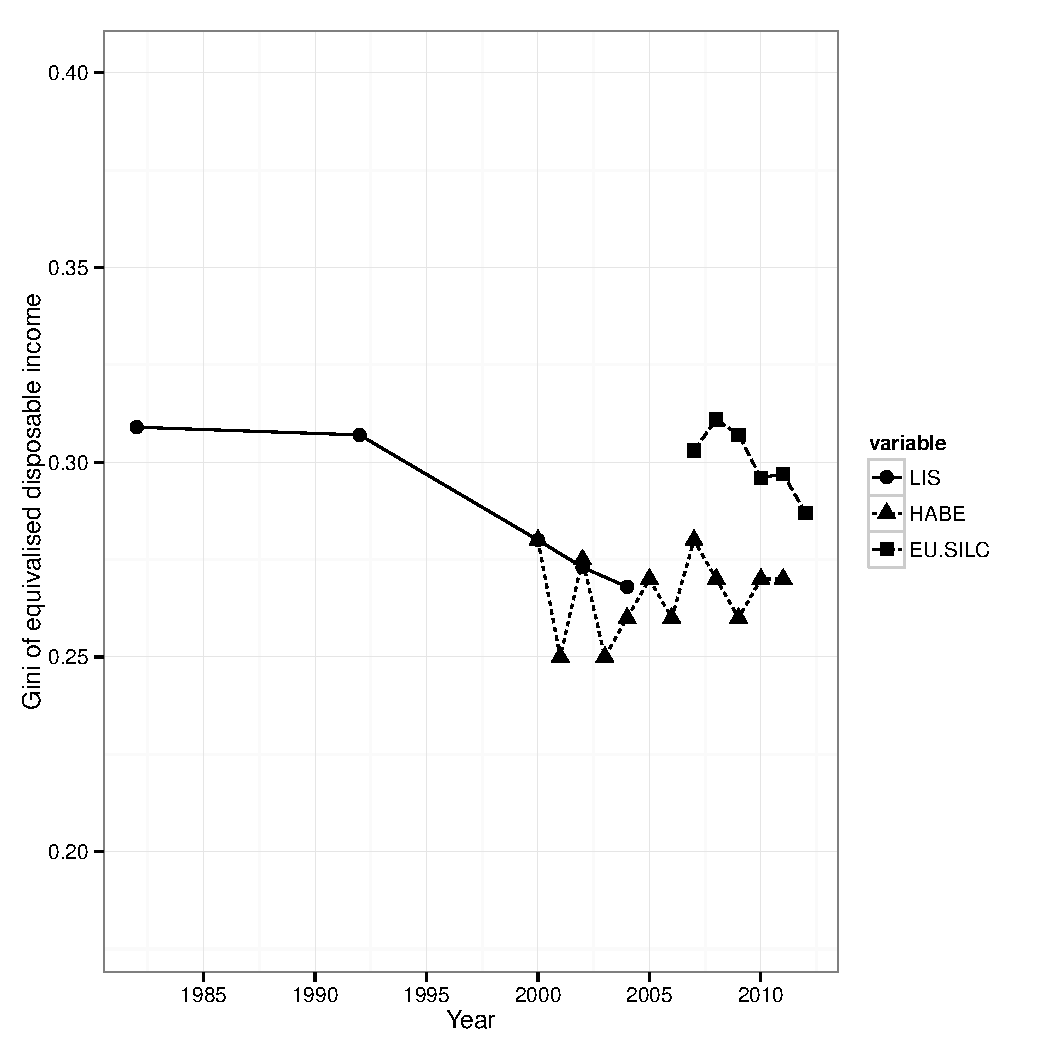
\includegraphics[width=\maxwidth]{figure/Swiss_inequality_Plot} 

\end{knitrout}


% 5.Abschnitt: What do we know about Switzerland
% Studies with tax data

Whereas the aforementioned publications focused on disposable household income from survey data, the revival of tax-data-inequality studies lead to fruitful insights for Switzerland as well. Dell et al. (2007) used tax data from the Federal Tax Administration to assess the development of concentration of the highest incomes and wealth (top-shares). In contrast to most other examined countries, Switzerland did not experience a reduction in income and wealth concentration from the pre-First World War period to the decades following the second World War (up to 1996). Using the same approach Foellmi and Martinez (2013) expand the Dell et al. timeline to 2008 finding that the share of top income has risen, the top 0.01\% share even doubled in the last observed 20 years. A result which opposes the outcome of official data published by the Swiss Federal Statistical Office.\footnote{There are other studies on Switzerland covering different periods but not the recent years. Flückiger et al. (2007) and also Jeitziner and Peters (2007,2009) report constant inequality from 1960-1996 respectively from 1995 to 2003. Covering a similar time period Bauer and Spycher (1994) and Bolzani and Abul Naga (2002) found decreasing inequality. On the other hand Buchmann and Sacchi (1995) and Ernst et al. (2009) found an increase in the 1980s).} \\

% 



% 6. Abschnitt: Zwischenbilanz und Herausforderungen

The divergence can be explained with several factors. First of all, different data sources were used. The official data providers trust on survey data, whereas the later mentioned publications use tax data. It is assumed that the coverage of top incomes is better in tax data than it is in survey data (non-respondent bias), which is a crucial issue concerning inequality. On the other hand the focus on top income neglects other changes in the distribution of income as it is not possible to see, whether newer concerns like the "hollowing of the middle class" occurred in Switzerland or not, which leads to the second point. Different measure of inequality hampers the comparability. Third, different income concepts and different units of analysis were used. As it is shown by Modetta and Müller (2012) income distribution is strongly affected by governmental redistribution, reducing inequality substantially. With the focus on tax data the change in institutional settings is not covered. Also neglected is the household structure, whereas it is unclear how inequality is affected whether one looks at household income or at income of tax units. It can be assumed, that inequality corresponding to different concepts react differently on demographic change (change in household structure). \\


% Allenfalls hier noch nicht so ausführlich mit Vor- und Nachteilen von Steuerdaten kommen. Vielleicht besser darauf hinweisen, welche Dimensionen betroffen sind und das dies in der Methods Section besprochen wird.
%rf: finde den abschnitt super

While there are several studies about income inequality in Switzerland, the publications concerning the distribution of wealth are scarcer, albeit the distribution of wealth seems to be a relevant dimension shaping the economic well-being of individuals as well. The cross-national Data center in Luxembourg is expanding their efforts, constructing the first cross-national wealth database. But, up to the day information for Switzerland is not available. 




% ab hier wird es irgnediwe unklar
Shorrock et al. (2013) unify several datasources (including tax data) to assess the pattern of global wealth. Their databook includes figures for Switzerland. In contrast to inequality of income concerning inequality of wealth Switzerland takes a leading position \\

% Albeit the awarness of an assessment of income and wealth simuntanously is rising, we focus in this paper on income inequality, which is the know as the core driver of economic inequlity
% Dann lassen sich einige Passagen streichen. Man könnte auch auf verschiedene Publikationen verweisen, welche die Bedeutung von Vermögen untersuchen -> Buch von Piketty, Müller und Schoch und dann aber ziemlich schnell darauf verweisen, dass wir uns hier auf Einkommen konzentrieren.
% Auch erste Dell Studie erwähnen -> es hat Zahlen zur Schweiz. Auch Probleme erwähnen (Fehlende Informationen zu Altersvorsorgevermögen -> hat aber niemand eine Lösung bisher.)
% Studies on inequality have to adress several thorny challenges. One has to define the centrale measure of inequality and find adquate data. Recent studies accentuate the importance of a broader concept of economic wellbeeing including measures for income, consumption and wealth alike. But each area is confronted with own measurement problems. Measure of consumptions are largely missing in tax data, albeit deductions can be understood as mandatory consumptions somehow. Measures of wealth are included in tax data, but are not connectable to the respctive income and therefore can only be analyzed separate. In danger of falling a pittraps it seems appriate to move in small steps. Therefore we focus our analysis on income, which is undoubtly a crucial indicator of economic wellbeeing.
% Also the Federal Statistical Office is increasing their effort to get sound data concering the distribution of wealth vgl. Müller und Schoch (2014).


% Zusammenfassung Stand der Forschung und festlegen unserer Ausrichtung

Up to the day, Switzerland can be situated according to the actual level of income inequality in western societies as there is a huge effort to collect data which can be harmonized to comparable measures (see Luxembourg income study, EU-SILC). However, it is unclear how the bias through non-response affects the overall measure of inequality. Likewise a long and consistent time-series allowing to identify and explore development patterns on every point of the distribution (not only the top-shares) and a time series for inequality of wealth is missing. Building on recent developments in the field of inequality research, we assess the suitability of the publicly accessible tax data to report inequality and its changes over time. First of all this includes a discussion of the accessible measures in context of a reflection about the state of the art conceptualization of economic resources as an indicator for economic well-being. Second, we summarize and apply tax data specific technics to construct suitable measures of inequality. We expand the given set by an in depth discussion of a newly applied step to handle the incomplete coverage in tax data statistics. Third, we integrate the development of Swiss inequality into the international picture.

% delete passages about wealth and include passage about the comparison with survey data

% Should we discus the non-scientic literature? -> allgemeine Frage und im konkreten betrifft dies die Publikationen von Economie Swiss und des Gewerkschaftsbunds.
% rf: gute frage, spontan würde ich sagen eher nein, müssten wir mal diskutieren


% Was wollen wir wissen?
% Wir müssen uns äussern zu: 
% Analyseinheiten
% Definition des Einkommens
% Berechnungsschritten

% Bei den Ergebnissen müsste es Grafiken haben zu:
% 1) Unterschiedlichen Analyseneinheiten (Mit und ohne Nuller, Normal- und Sonderfälle)
% 2) Unterschiedliche Einkommensgrössen (Reineinkommen, steuerbares Einkommen, pseudoverfügbares Einkommen (Abzüge von direkten Bundessteuern))
% 3) Vergleich mit HABE 












%%%-------------------------------------------------%%%
%%% How did inequality change over time %%%
%%%-------------------------------------------------%%%

%<<subdoc_content_introduction, child='subdocuments/change.Rnw', eval=T>>=
%@

% Section from an older version. Currently disabled.


%%%-------------------------------------------------%%%
%%% Include data and methods %%%
%%%-------------------------------------------------%%%


%%%-------------------------------------------------%%%
%%% Sub document for data and methods %%%
%%%-------------------------------------------------%%%

\section{Measurement concepts, Data and Methods}

To discuss the suitability of a specific data source it is crucial to have an idea about an ideal measure. Based on a review on the literature about the measurement concepts in an ideal world, we discuss briefly the advantages and shortcomings of tax data compared to other data sources - namely survey data. Afterwards we describe the tax data published by the Swiss Federal Tax Administration highlighting the important aspects, which have to be considered working with FTA-Data. In the last section, we describe the methods and corrections we used to construct the time-series of inequality-measure for income an wealth for Switzerland.

\subsection{Standards for measuring economic resources and inequality}

\emph{Concepts on measuring economic resources}  \\
Most studies on inequality focus on income inequality, while economic resources are ideally conceptualized with measures for income, wealth and consumption together. In generall it has to be stateted, that ideal measures only can be defined in context of a given reaserach question. This holds, if one thinks about the ideal measure of economic well-being, but also about the unit of analysis. Nevertheless, some more or less unified concepts exists, which can be taken as a starting point. OECD (2013) \\

% We neither can examine consumption nor the jointly distribution of income and wealth on the individual level. We could analyse the jointly pattern on the cantonal level and analze the data following the question if income inequality and wealth inqueality are correlated.

\emph{Defining income}

\begin{itemize}
\item Market income refers to revenue from employment.
\item primary income or pre-transfer income refers to  market income plus revenue from property (capital income)
\item Brutto income refers to  primary income plus social transfer
\item Disposable income or posttransfer income refers to  brutto income minus transfer paid 
\item adjusted disposable income refers to  disposable income corrected for the numbers of household members 
\end{itemize}

The appropriateness of the income concept is bound to the research interest. Studies focusing on labor market outcome look at market income. Studies focusing on human wellbeing follow the approach as propagated by the oecd (2013). This concept is largely implemented by the Federal Office of statistics. Following this concept one should look at income after taxes and transfers inclusive the adjustment for household members, because this is the measure which frames the consumption possibilities. Lastly, studies focusing on the effect of institutions (social welfare, taxation) compare the distribution of pre- and post-income measures. \\   

% an income which is adjusted for the household size is not a real income anymore. It is a measure of indivdual welfare or of the standard of living (BFS:2012)


\emph{Defining wealth}
While the apropiateness of the conceptualization of income is widely discuded, there is no agreed definition of personal wealth yet and the appropriate methods of valuation are not always clear. 
Wealth can be defined as the marketable value of financial assets plus non-financial assets (housing and land) less debts (Credit Suisse 2011:5).

% Streichen

\emph{Population Coverage} \\
All Residents? Working Residents? Single Person vs household/family. Households without income \\
see for details: OCED Framework for Statistics on the Distribution of Houshold income, consumption and wealth (2013) \\

The income of the household generally plays the major role in the living standards attained by its members, so the way earners and non-earners grouped together in households, has to be incorporated into the analysis. Especially when the the focus of interesst lays in unrevealing the role of demographic factors. 


\emph{Measuring inequality and concentration} \\
To be able to make qualifying statements about a distribution or to compare different distributions, the concept of inequality turned out to be the most appropriate and thus the most commonly used dimension. Vgl. Allison (1978), Engelhardt (2000), Cowell (2000) oder Hao/Naiman (2010)
%[Zusammenfassung bestehender Überlegung und Hinleitung zu den Masszahlen, die wir verwenden werden (vermutlich Gini und relative distribution methods) \\

neuere Indikatoren; Polaritätsindex: relative distribution methods in the Social Sciences (Handcock/Morris 1999) \\

Gini is mainly used for international comparison. However, other measures are often reported along (gini is more sensitive to changes in the middle of the distribution than to changes in the tails (OECD, 2008:37). Newer branches of inequality studies emphasize the need for broader measures of inequality, which allow better analyses about the change of inequality and namely statements about the area of change (downgrading/upgrading) (Alderson and Doran 2013). \\

Alvaredo (2010) shows formally, how top incomes shares are related to the gini-coefficient. Following his argument, it is crucial to consider top incomes. Leigh (2007) also analyzed the relationship between the Gini (and further inequality measures) and top income shares in a panel of 13 countries (Switzerland is part of the studie). 
%[He also discusses tax data studies in general-> have a closer look] \\
%[We definitely have to argue, why it isn’t sufficient to report top income shares, because if it is, there is no need to have another study about Switzerland (national level>Martinez, cantonal level> gorgas and Schaltenegger)]

\subsection{Comparison of tax data and other data sources - advantages and shortcomings}

% Suitability of data sources can be judeged by different criterias. crossectional or longidutional perspective. longidutional perspective allows for dynamic 

%[ich stelle mir eine Tabelle mit verschiedenen Dimensionen vor, anhand derer eine Einordnung unterschiedlicher Datenquellen geschieht.]
% Mögliche Vergleichsdimensionen
%- Suitability of cross country comparison
%- Coverage of the population of interesst
%- Implementation of common concepts of economic ressources
%- contingency for intertemporal comparision

%Burkhauser et al. (2009) compare inequality statistics form survey data and tax records to consolidate the findings about recent trends in the USA

%Warnings about the use of tax data
%The use of tax data is often regarded by economists with considerable disbelief. These doubts are well justified for at least two reasons. The first is that tax data are collected as part of an administrative process, which is not tailored to the scientists' needs, so that the definition of income, income unit, etc., are not necessarily those that we would have chosen. This causes particular difficulties for comparisons across countries, but also for time-series analysis where there have been substantial changes in the tax system, such as the moves to and from the joint taxation of couples. Secondly, it is obvious that those paying tax have a financial incentive to present their affairs in a way that reduces tax liabilities. There is tax avoidance and tax evasion. The rich, in particular, have a strong incentive to understate their taxable incomes. Those with wealth take steps to ensure that the return comes in the form of asset appreciation, typically taxed at lower rates or not at all. Those with high salaries seek to ensure that part of their remuneration comes in forms, such as fringe benefits or stock-options which receive favorable tax treatment. Both groups may make use of tax havens that allow income to be moved beyond the reach of the national tax net. These shortcomings limit what can be said from tax data, but this does not mean that the data are worthless. Like all economic data, they measure with error the 'true' variable in which we are interested.
%The data series presented here are fairly homogenous across countries, annual, long-run, and broken down by income source for several cases. Users should be aware also about their limitations. Firstly, the series measure only top income shares and hence are silent on how inequality evolves elsewhere in the distribution [why?]. Secondly, the series are largely concerned with gross incomes before tax. Thirdly, the definition of income and the unit of observation (the individual vs. the family) vary across countries making comparability of levels across countries more difficult. Even within a country, there are breaks in comparability that arise because of changes in tax legislation affecting the definition of income, although most studies try to correct for such changes to create homogenous series. Finally and perhaps most important, the series might be biased because of tax avoidance and tax evasion. For the details, we refer users to the original papers (see also Atkinson, Piketty and Saez, 2011).

%Copied from:
%Alvaredo, Facundo, Anthony B. Atkinson, Thomas Piketty and Emmanuel Saez, The World Top Incomes Database, http://topincomes.g-mond.parisschoolofeconomics.eu/ , 18/12/2013

\textbf{Summary of tax data drawbacks}
\begin{itemize}
\item Misreporting of incomes (high earners have an interest in getting tax beneficial "income" see above)
\item with aggregated data the adjustment for household members is not possible (no equivalization possible). This is a point, which is hardly mentioned in the "top-income" literature, albeit it is a crucial issue in "theorized" concepts of income. To generalize one can say, that the concept of tax units (individuals and couples + no direct information about household members at least not in the aggregated tax tables) is not congruent with the concept of household. This might influence the overall inequality, taking into account the change from traditional household and family structures over the last century. This is an inequality related issue, where relevant studies are missing. What are the assumptions?
\item the tax data income definition summarize labor income, capital income and taxable transfer payments (no means-tested benefits as welfare aid). Distinction between the different income sources is not possible, albeit the mechanisms of changes in the specific distribution can be very different.
\item Some tax units are not included in the tax tables (see Foellmi and Martinez 2013:11f).(a) only taxed cases are included (partly a problem, for certain periodes we know how many cases are excluded because of low or none income)	- (b) cases tax at source (Quellenbesteuerung). Foreign nationals living in Switzerland but with a yearly or any other temporary resident permit only. In some border-cantons the share of this group is very high (20\%) 
%Can we ignore this)
(c) staff of international organizations based in Switzerland	- (d) non-fillers show up in the tables as long as they are registred. This persons get an imputed income (older tax tax return and information given by employers. Not registered non-	fillers are not in the records.
- (e) tax evasion. Feld and Frey (2007) report about tax evasion in Switzerland, it should be somewhat above 20 percent on average. With the (strong) assumption that the pattern of tax evasion over time is stable, this is a minor problem for inequaly measures over time.
\end{itemize}

\textbf{Problems with household income surveys}
\begin{itemize}
\item Sample data (bias)
\item comparability between countries and over time (depends on income definition)
\item short time series
\end{itemize}

Atkinson et al. (2009) estimate that CPS survey data fail to capture about half of the overall increase in inequality measured by the Gini coefficient, a result confirmed by Alvaredo (2010). \\

See for other countries: Siminski et al 2003 (Australia), Brewer et al 2008, UK, Burkhauser et al. 2009, US)
%	•	What about the special cases? Foelmi and Martinez argue, that it is crucial to include the special cases because they include the high net wealth individuals taxed according to their expenditures. Exclusion leads to an underestimation of inequality
%	•	Capital gains? Should not be included 
The discussion about problems with reporting income is fairly exhaustive. What about wealth?

It is well recognized that the traditional sources of wealth distribution data are unlikely to provide an accurate picture of wealth ownership in the top-tail of the distribution. Credit Suisse (2011) makes use of the information in the "Rich Lists" published by Forbes Magazine to adjust the wealth distribution pattern in the highest wealth ranges. \\

Additonaly the Credit Suisse Reports states (2011:8) that these data my be less subject to response bias, but my be more prone to valuation problems, especially in connection with pension assets and debts.

\subsection{Tax data published by the Swiss Federal Tax Administration}

%Beschreiben was die Daten beinhalten und wo es Probleme gibt
\begin{itemize}
\item	Datengrundlage: 1947/48 bis 1981/1982 Eidg. Wehrsteuer. 1983/1984 bis 2010 direkte Bundessteuer. Zugänglich über estv.admin.ch
	\item	Special feature Switch from bi-annual taxation to standard annual tax-system (1995/1996 bis 2003)
	\item	Tabulation by size of income and statistical measures from individual tax records (Brülhart-Daten)
	\item	Income after deductions-> taxable income (employment income, business income and capital income). Is income definition stable over time? Yes it should. Realized capital gains are excluded from the definition. It includes income from  employment, self-employment, capital income and taxable transfer payments. Plus Eigenmietwert, 
	\item	Reported on national and cantonal level
\end{itemize}

\subsection{Ways to tackle FTA-tax data specific problems}

\textbf{Incomplete coverage of the population (left censored data.)} What can be done about the not-taxed? Del et al. (2007) impute for non-fillers the 20 percentage of the annual average income. This flattens the distribution on the left side, which is not a problem if you are interested in the top income shares, but it would surly affect overall measures of inequality. Furthermore Del et al. calculate the proportion of non-fillers by estimating the total of tax units out of the population records. \\

\textbf{changes in taxation system  (switch from annual to biannual taxation)} In the mid-1990s a fundamental change in the Swiss tax system took place by switching form the two-years based praenumerando taxation to the one-year based postnumerando taxation. This change was enacted with a transitional period of several years, during which each canton could choose when to adopt the new system.  This is why during the transitional period from 1995 to 2003 there is no uniform tax data published on the Swiss level but only data on the cantonal level  (Foellmi and Martinez:8f). \\
%es wird erwartet, dass der Wechsel Ungleichheitsmasse beeinflussen. Yearly fluctuations are dampened, when income is measured on a two-yearly basis.

\textbf{Estimating percentiles from bracket income tabulation} Pareto interpolation \\ 

\textbf{Missing of mean-tested benefits as part of the income} -> imputation with recommendation for minimum level for basic needs defined by the SKOS.\\
%is never mentioned as a problem, but it seems to me a better way to approach the non-taxed issue, than dell way (20 % of average income)

\textbf{deductions} Del et al. (2007:477):" we can check with statistics for 1971-72 (as well as later years) presented both by size of income before deductions and income after deductions that adding back deductions does not introduce any significant error in our estimates."
Gorgas and Schaltenegger (2011:5): "..., information on [...] deductions is provided in the tax statistics, thus, we could add the personal deductions to the income data to obtain a consistent series over time". Können wir das auch? Zumindest für gewisse Zeiträume? Das wäre noch gut. \\

Studies on income try to focus on the disposable income, which subtracts certain expenditures from the primary income. Deductions reflect somehow compulsory expenditures and thus taxable income can be seen as a sort of pseudo disposable income. On the other hand deductions can affect the distribution. There are recent studies about the correlation of progressivity and deductions in Switzerland, which examines if deductions have a "perverse redistribution" effect by redistributing income from the lower middle class to the upper middle class (vgl. Peters 2011 and Interpellation Barbara Gysel (2009).

% Income share specific problems
% Total income denominator Exogenous Approach -> net income reported in the national accounts. Endogenous Approach -> Dell et al. technic-> imputing 20\% of average personal income to non-fillers (which are mainly persons with low or no income). Honestly , is this appropriate? (Everyone did it)
% Total of tax units in the country. exogenous approach -> construct number of total tax units artificially from other data sources
% Endogenous approach -> reported in the tax tables 

%%%-------------------------------------------------%%%
%%% Abschnitte aus ersten Version des Papers %%%
%%%-------------------------------------------------%%%

%\subsection{Hypotheses}
%Based on the theories we test the following hypotheses:

%\begin{itemize}
%\item H1: Develpment of inequality is driven by sectoral change
%\item H2: Development of inequality is driven by political change, i.e. economic crisis contribute to inequality because welfare states tend to be downsized
%\end{itemize}

%\subsection{Data and Variables}

%We use data from the Swiss Federat Tax Administration (FTA) where our data about incomes ranges from the years 1941/42 to 2010. While the data results in a long and consistent time series to illustrate swiss inequality development, there are a few pitfalls we want to adress which might be of interest for other research on this topic (be it in Switzerland or other countries).

%\subsubsection{Left censored data}

%The FTA provides data about all tax units in Switzerland that are liable to pay federal taxes.A tax unit may be a single person or a household. The taxable population however is not identical to the population which should be used to calculate measures of inequality. Precisely, the data do not contain tax units with very little incomes so calculations based on these data treat the lowest percentiles equally to tax units with zero income.Figure X shows the threshold to be hit to enter the statistic.

%\textcolor{red}{[FIGURE X ABOUT HERE] soll zeigen: Zeitreihe der Untergrenze von 1941-2010}

%So first of all, there is a bias in the level of an inequality measure one could calculate with the   FTA data. Furthermore, also the changes over time might not be interpreted savely as over time the number of tax unit within this "hidden range" might vary or might even have a certain trend. We will adress this issue in detail in the methods chapter.

%\subsubsection{Different measures, different populations}

%The FTA data makes two kinds of distinctions. First, data was collected for so called "normal cases" and "special cases", i.e. a "normal case" is a taxable (for the complete tax period) person or household domiciled in a swiss canton without income from outside of Switzerland. A "special case" therefore is a diffuse reference category that contains tax units that are taxed at source, were not taxable for the complete tax period or generated additional income in another country. Second, the FTA reports two measures, that is taxable income and absolute income \textcolor{red}{(meine vorläufige Übersetzung von Reineinkommen)}. Absolute income is the sum of all incomes (earnings, interest income, rental incomes) minus expenses (e.g. from self-employment or credit cost). The taxable income is calculated as the difference of absolute income and deductions (e.g. children, insurance rates). The longest consistent time series exists for the taxable income of normal cases. So all statements we make with our data only apply to this subpopulation.

%\subsubsection{Changes in taxation and measurement}
%The swiss tax system is highly federal. That means, communities raise taxes which then go to the communities, the canton and the state. If we want to calculate overall swiss measures, we need to take into account, that cantons vary (between cantons and over time) with regard to the tax deductions that are possible and also the mechanism how taxes are collected. The latter adresses a comprehensive reorganization of the swiss tax system where between 1995 and 2003 cantons changed from taxing the past two years of income (postnumerando system) to taxing the present single year (praenumerando system). For details see \textcolor{red}{Martinez (xxxx) or some other author (xxxx)}. Aggregate measures of inequality therefore have to be estimated for the periods 1995 to 2003 which we adress shortly in the methods chapter.

%\subsection{Methodology Used}
%There are two steps of data analyses which need to be described to the reader. First, the estimation of the bias we introduce by estimating measures of inequality when tax units with too little income are not observed. Second, the steps undertaken to estimate aggregate swiss measures by imputing taxable income for those cantons and periods where the change of the tax system produced a gap (1995 to 2003, depending on the canton). 

%\subsubsection{Imputing the gap}
%The imputation is not a focus of the paper so we basically follow the most simple approach of Martinez (xxxx). That is estimating the missing taxable income statistics via OLS using information from time trends and cantons. Our imputation model therefore includes canton inequality measures and periods dummies to explain aggregate swiss inequality.

\subsubsection{Estimating the bias}
For most of the observed range (1941 to 2010) we do not have any information how many tax units fall into the category of having income that is not zero but is too little to qualify for federal taxation (lets call those "zeros" for convenience) . However starting 1995, the FTA provides exactly this information for each canton. This enables us to estimate the bias we introduce for each canton and each period between 1995 and 2010. Consequently we can obtain information whether the bias is stable over time (which makes it possible to safely interpret the changes of inequality over time) and whether the bias is different for each canton. \textcolor{red}{Unterschiede zwischen Kantonen wären gut um zu argumentieren, dass andere Länder auch davon betroffen sind, in etwa sowas wie "je höher der Steuerfreibetrag, umso stärker der Bias". Länder de erst sehr spät besteuern (und über nicht Besteuerte dann auch nicht Buch führen) haben einen krassen Bias. Wir könnten dann empfehlungen geben, ab welchem Perzentil man save interpretieren kann oder so.}

One can take a first look at the descriptives plotting the share of zeros over time seperately for each canton .




\begin{knitrout}
\definecolor{shadecolor}{rgb}{0.969, 0.969, 0.969}\color{fgcolor}
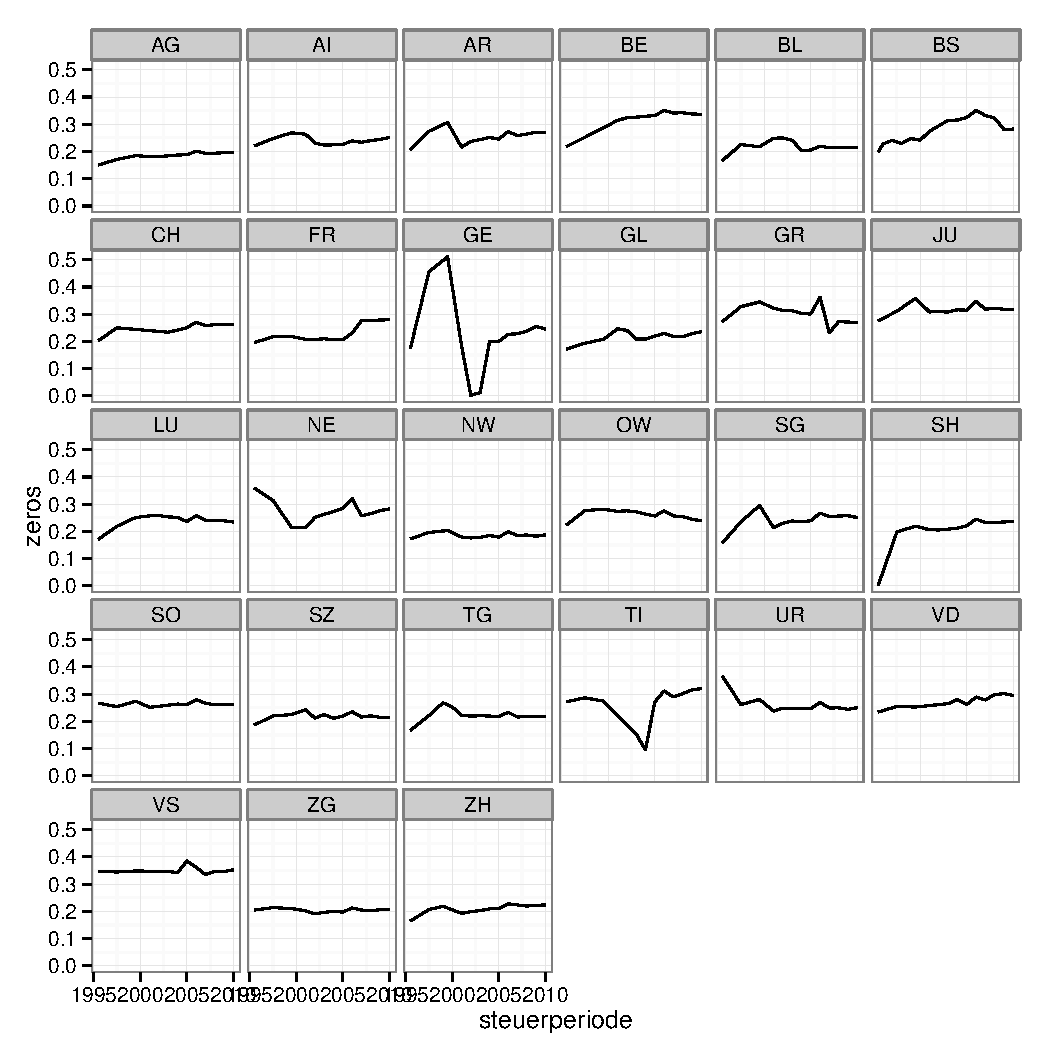
\includegraphics[width=\maxwidth]{figure/zero_descriptives1} 

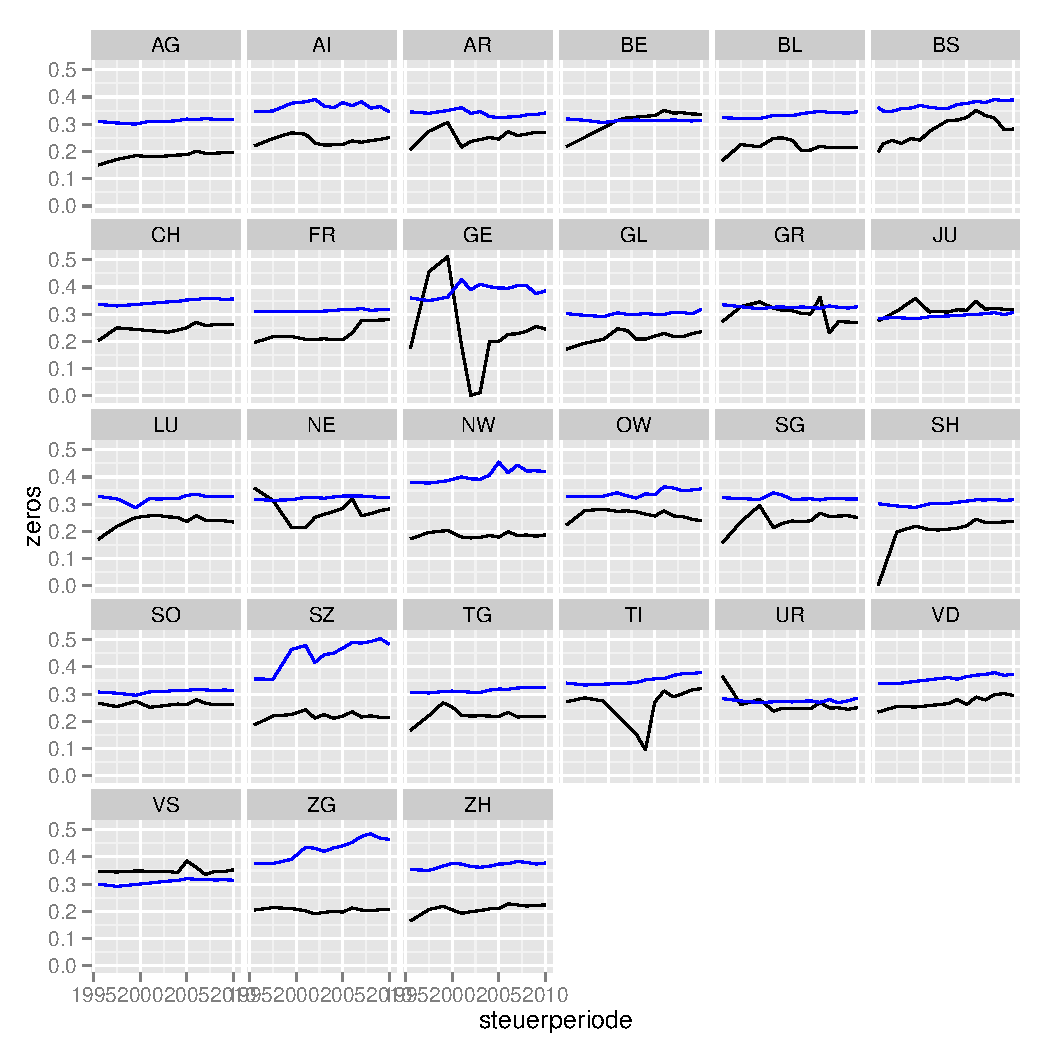
\includegraphics[width=\maxwidth]{figure/zero_descriptives2} 

\end{knitrout}


We can see multiple things here:

\begin{enumerate}
\item There is a small overall upward trend which we assume to be the Federal Administrations inflation adjustments to the tax threshold.
\item Geneva and Tessin show wild changes but those might be explained by the tax gap ("Bemessungslücke") that people exploited when the cantons changed the tax system. It remains unclear however why we can't see similar patter within other cantons.
\item There is some variance and we see different patterns over time and cantons. When estimating gini coefficients or the like we must therefore assume that ignoring "the zeros" leads to a bias that is not stable over time.
\end{enumerate}

We might try two strategies to moderate the problem:

\begin{enumerate}
\item Add the zeros as a seperate group
\item Fit a model to predict the inequality measure (e.g. the gini coefficient) using the share of zeros as a predictor
\end{enumerate}

By adding the zeros as a seperate group we face several problems. With the exception of Geneva 1995/96 Pareto interpolation of percentiles p20 and above seems viable. Low percentiles however would need to be extrapolated so we might impose unrealistic assuptioms. Even when estimating "safe" measures above p20 (better p50) or a gini coefficient we need to make an assumption about the income structure of that group (a distribution, a mean income or zero-income). To be consistent with the measure of "taxable income" we could assume an income of zero for that group, calculate gini coefficients and compare them with the original (uncorrected/plain) version. To get a rough number we could (cantonwise) check the squared correlation between plain and corrected gini.

The second approach however is more robust as we do not impose additional assumptions but instead exercise some curve fitting.

\begin{knitrout}
\definecolor{shadecolor}{rgb}{0.969, 0.969, 0.969}\color{fgcolor}
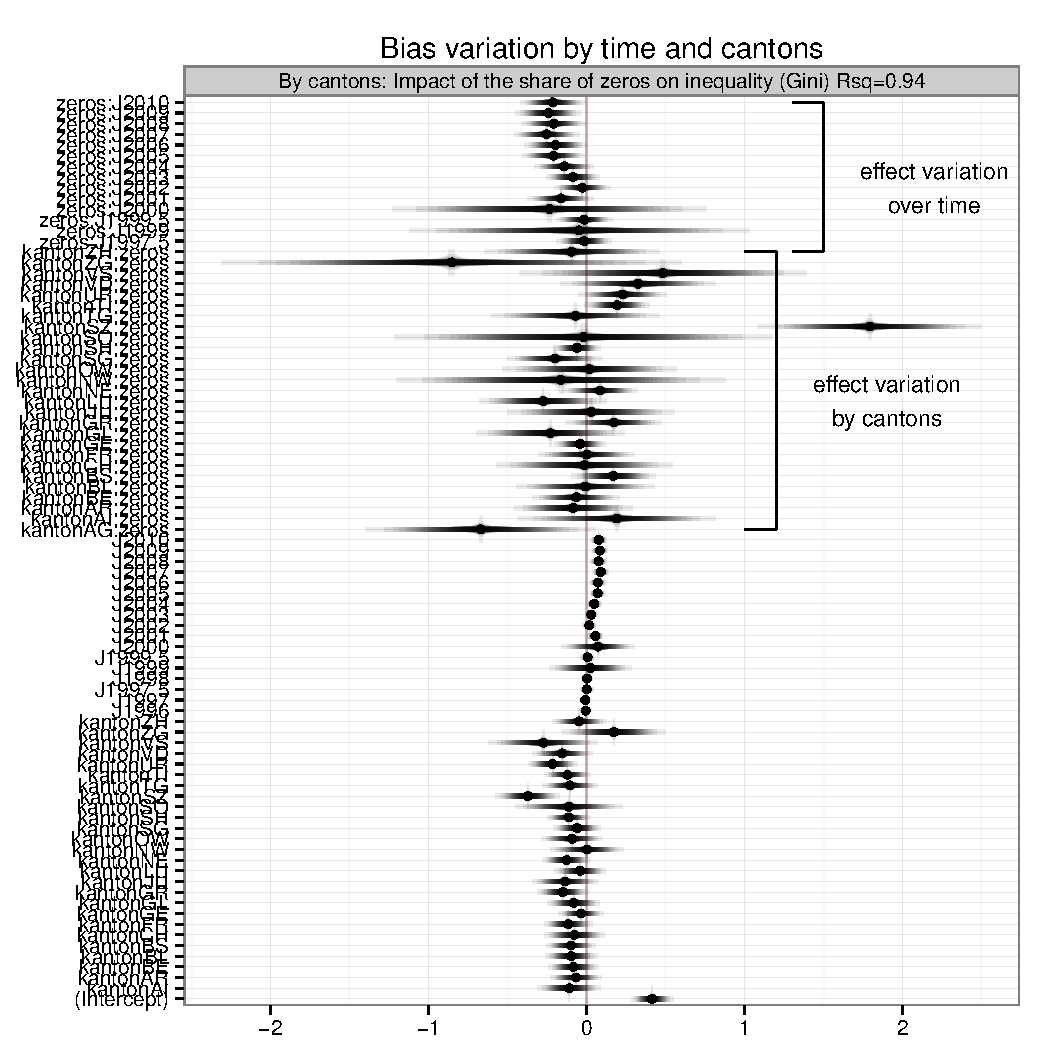
\includegraphics[width=\maxwidth]{figure/corrected_gini} 

\end{knitrout}


The model outputs a test statisic for each canton that tells us whether the variation of the zero-rate over time leads to a significant deviation from the typical "canton gini-level". As the model has a decent fit we are not in great danger of omitted variable bias. Using a joint F-Test we can now test if all canton#zeros interactions are zero. 

\begin{knitrout}
\definecolor{shadecolor}{rgb}{0.969, 0.969, 0.969}\color{fgcolor}\begin{kframe}


{\ttfamily\noindent\itshape\color{messagecolor}{\#\# \\\#\# Attaching package: 'survey'\\\#\# \\\#\# Das folgende Objekt ist maskiert from 'package:graphics':\\\#\# \\\#\#\ \ \ \  dotchart}}\begin{verbatim}
## Wald test for kanton:zeros
##  in lm(formula = G_steink ~ kanton + kanton:zeros + J + zeros:J, 
##     data = df)
## F =  3.282  on  27  and  262  df: p= 4e-07
\end{verbatim}
\end{kframe}
\end{knitrout}


In our case we can clearly reject the hypothesis that all interactions are zero. This leads to the conclusion  that gini coefficients are biased by the variation of the zero-share which is kind of obvious but at the same time we can use the model to report adjusted gini coefficients. For example one might be interested in how inequality would had developed if the zero-share would have been constant over time. (Note RF: predict all data point using canton, time and the initial OR final zero-share to homogenize the time series)
Furthermore we can quantify how large the bias is and we can do this seperately for tax periods or seperately for cantons. 

For all cantons:




We can see the the model fit reduces to explaining 61.5\% of the gini variation versus 92.6\% when the information from the zero-shares was used. Although this so some extent attributable to the additional 26 paramters: this is huge. 

The model indicates some cases that deserve more attention: Schwyz (positive coefficient) and Geneva (negative coefficient) and the tax period 2000 as well as the most recent periods.

A positive coefficient (e.g. Schwyz) can be read as follows: In periods with many zeros we measure higher gini coefficients. We can derive, that the distribution of income is more scewed for high incomes than for low incomes. Simply speaking, the contrast between low and middle class is less pronounced than the contrast between middle und high class. One possible explanation would be that incomes stem from two different populations: 1) the people of Schwyz who possibly follow a log-normal or gamma distribution and 2) particularly rich people who moved to Schwyz to avoid taxes. 

A negative coefficient (e.g. Geneva) means the more zeros there are the smaller the gini measure was compared to other tax periods within that canton (remember this is a fixed-effects model). This is the case we would usually expect: more zeros mask inequality that arises from the bottom.

What can we conclude from that analysis? First one must notice that aggregate measure like the gini (or others) do not always react in the same way when we cut off one part of the distribution, therefore the measures calculated from tax data is biased. On the other hand, the model coefficient of Switzerland as a whole is not significant suggesting that the cantonal biases cancel out each other. This seems plausible. Most of the "tax optimization" happens within Switzerland so the rich people who moved to Schwyz are now missing at another canton.

We can even see more from the model coefficients. The period dummies indicate how the distribution of incomes has changed: compared to 1995, the subsequent periods have a negative coefficient, i.e. the bias we introduce by omitting the zeros increased, especially from the mid nineties to the mid 2000s. To simplify: cutting off zeros more and more seems to lead to an underestimation of our inequality measure, probably because the skewness in the left part of the distribution increased pointing to an increased pauperization that is masked by omitting the left tail of the income distribution.




%%%-------------------------------------------------%%%
%%% Include results %%%
%%%-------------------------------------------------%%%


%%%-------------------------------------------------%%%
%%% Sub document results %%%
%%%-------------------------------------------------%%%

\section{Results}

\textcolor{red}{Gesamtschweizer Grafik (mit imputierten Daten) einmal eine Linie mit Bias, einmal ohne
Kantonsweise Grafiken
Kuznets / U-Turn, Test der Hypothesen mit den final Daten. Der link zwischen rein deskriptiv  und Theorie plus Modell ist aktuell noch ein krasser Drahtseilakt...}

\subsection{Gini coefficients for taxable income, income before deductions and taxable income after tax}




\begin{knitrout}
\definecolor{shadecolor}{rgb}{0.969, 0.969, 0.969}\color{fgcolor}\begin{kframe}


{\ttfamily\noindent\itshape\color{messagecolor}{\#\# \\\#\# Attaching package: 'reshape'\\\#\# \\\#\# Die folgenden Objekte sind maskiert from 'package:plyr':\\\#\# \\\#\#\ \ \ \  rename, round\_any}}\end{kframe}
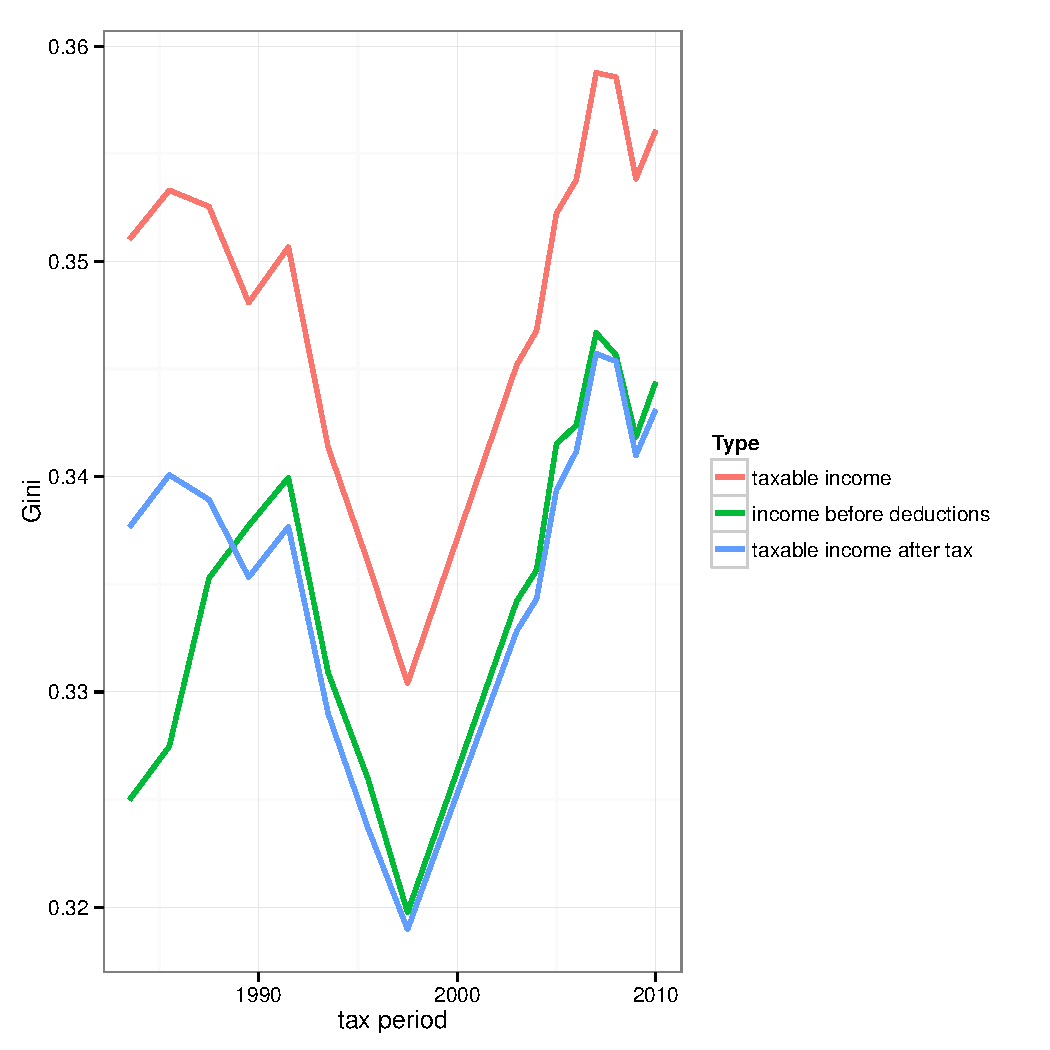
\includegraphics[width=\maxwidth]{figure/different_ginis1} 

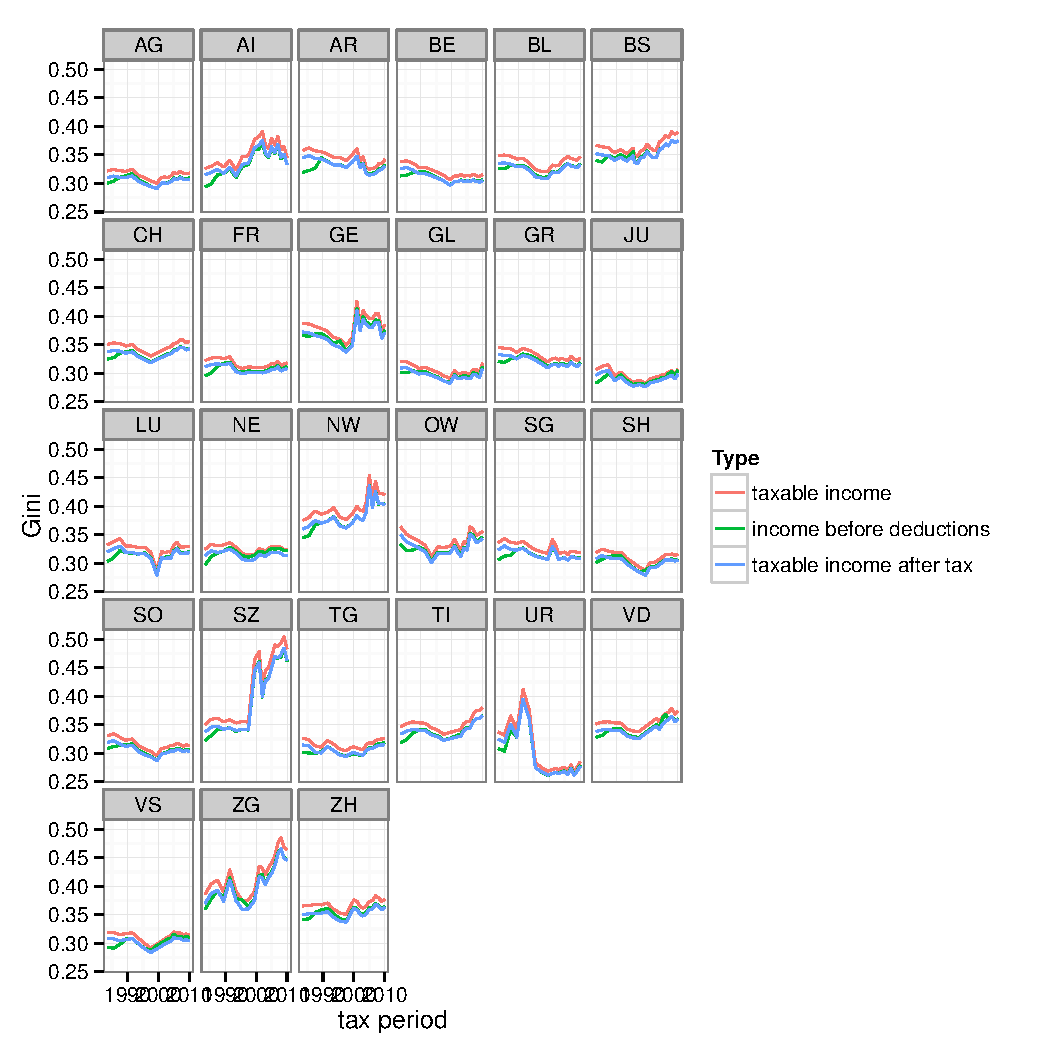
\includegraphics[width=\maxwidth]{figure/different_ginis2} 

\end{knitrout}


\subsection{Zero share}

Estimation using population statistics (1945/46-1993/94) and official tax administration statistics (1995/96 and later) 


\subsection{Income measures with and without zeros}

taxable income with and without zeros

\begin{knitrout}
\definecolor{shadecolor}{rgb}{0.969, 0.969, 0.969}\color{fgcolor}
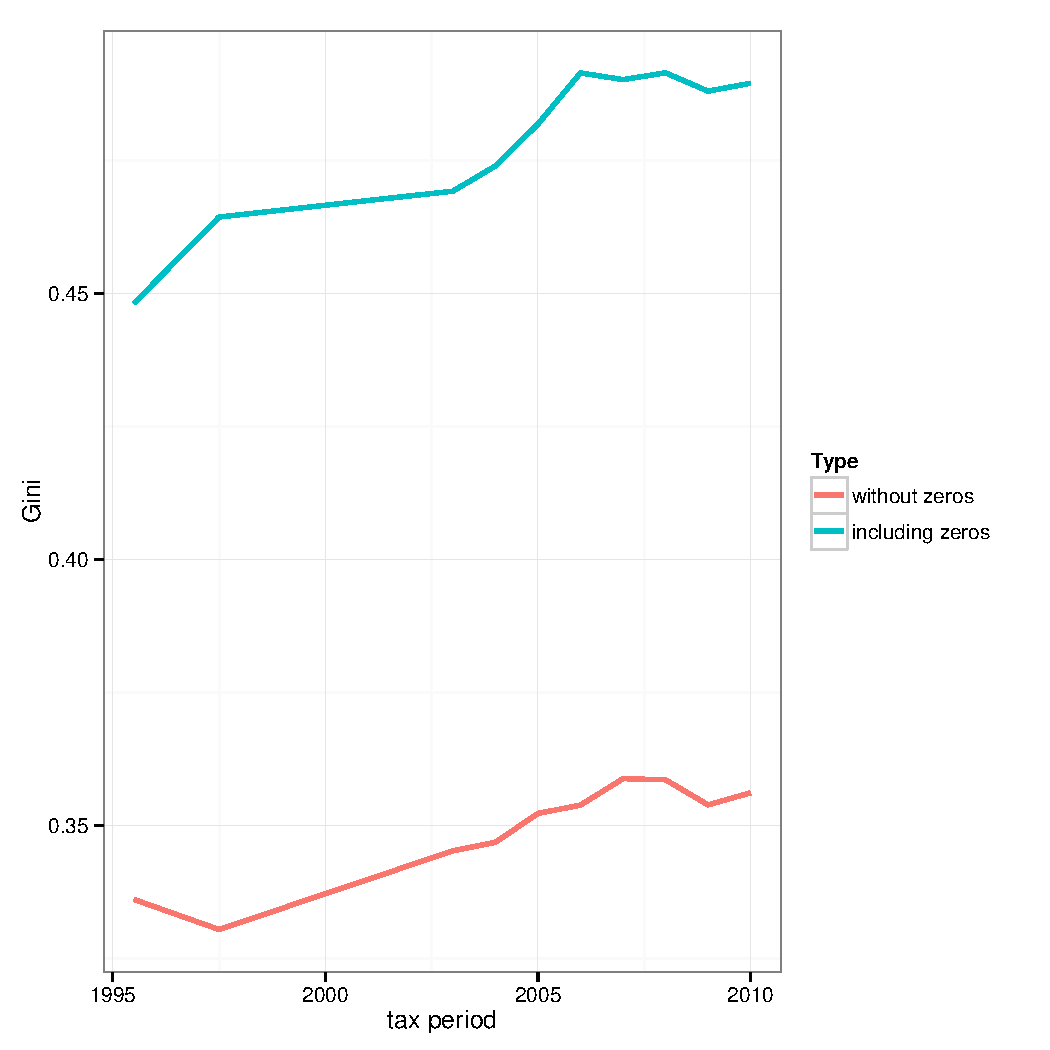
\includegraphics[width=\maxwidth]{figure/with_without_zeros1} 
\begin{kframe}

{\ttfamily\noindent\itshape\color{messagecolor}{\#\# 'opts' is deprecated. Use 'theme' instead. (Deprecated; last used in version 0.9.1)\\\#\# theme\_text is deprecated. Use 'element\_text' instead. (Deprecated; last used in version 0.9.1)}}\end{kframe}
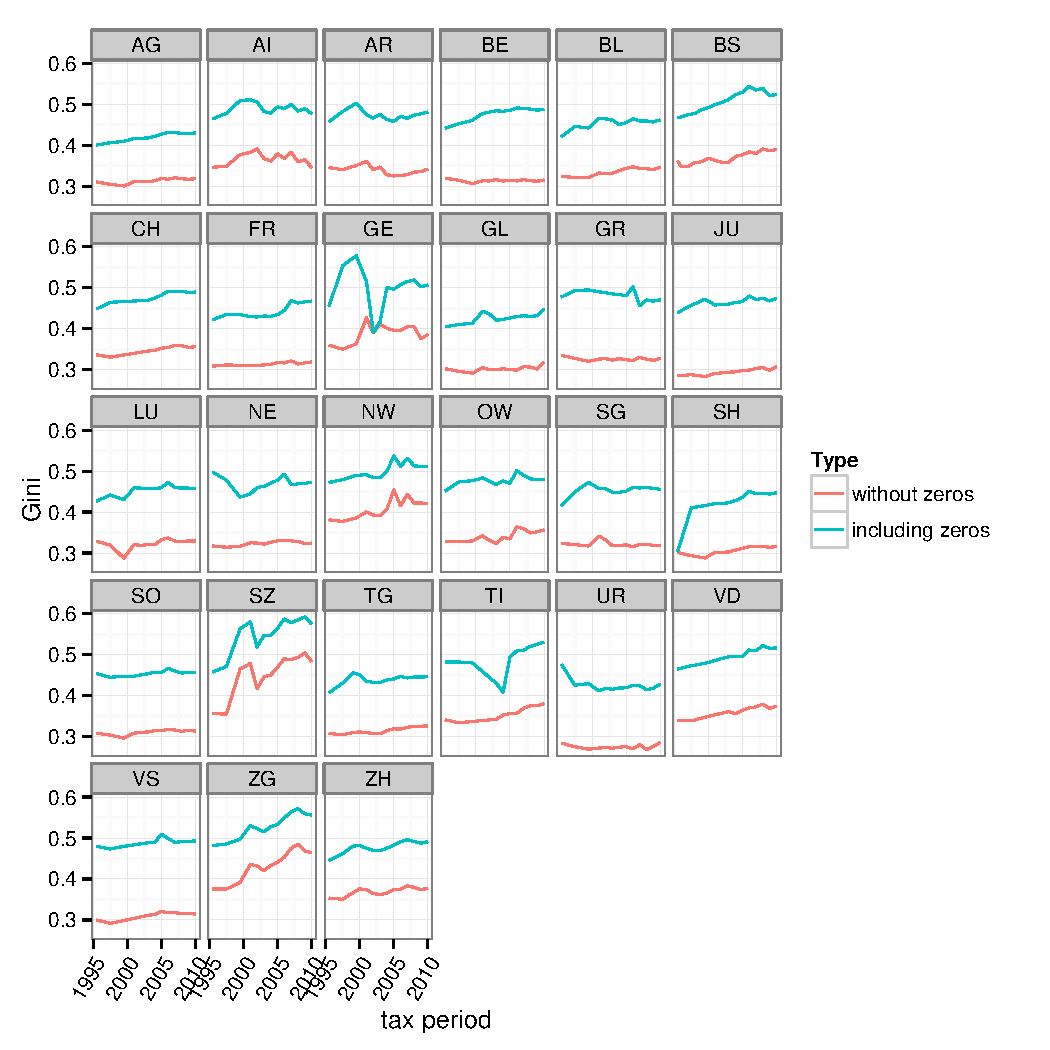
\includegraphics[width=\maxwidth]{figure/with_without_zeros2} 

\end{knitrout}


Including zeros leads to significantly higher gini coefficients. However we must keep in mind, that these might be artifically high values as we assume zero income for everyone in the zero group. We can conclude more from the graphic: the ratio between both measures seems to be quite constant although for aggregate Switzerland but there are minor deviations for multiple cantons as well as strong deviations for the cantons Geneva and Tessin. However the problems seem not to result from a shift in the zero-share over time but they are specific for the time-period when the tax system changed. 

%Switzerland (income and wealth)
%- graph with gini over time> identify periods of change
%- closer look at interesting periods with relative distribution methods-> is change because of down- or upgrading?
%Cantonal level (income and wealth)
%- different development on regional level 
%Switzerland in international comparison
%- Comparison with other data sources- LIS (inequality in Switzerland is decreasing, which is quite special, because the common pattern in western countries shows an increase in inequality

%- Comparison with other countries (similar data)


% Es scheinen mir aktuell etwas viele Ergebnisse zu sein und ich frage mich, ob wir Ergebnisse auf der Kantonsebene ausklammern sollen. Wenn wir drei Ergebniss haben (1) Unterscheidung von unterschiedlichen Perioden der Ungleichheitsentwicklung (2) Beurteilung dieser Perioden hinsichtlich dem Bereich der Veränderungen (Arme, Reiceh) und Entwicklung der Vermögensungleichheit, dann haben wir bereits viel. Falls wir spezifische Erkenntnisse nur aus dem Kantonsvergleich bekommen (Bias durch Nuller o.ä.), dann sollten wir trotzdem damit arbeiten.

%rf: genau. kantone unterstreichen die probleme mit dem 0er bias und die probleme mit "imputing the gap". mehr muss erstmal nicht sein.




%%%-------------------------------------------------%%%
%%% Include discussion %%%
%%%-------------------------------------------------%%%


%%%-------------------------------------------------%%%
%%% Sub document for discussion %%%
%%%-------------------------------------------------%%%

\section{Discussion}

% Hier könnte allenfalls der Bogen zur Theorie gespannt werden 

%Methodological Main findings 
%(1) Tax data is useful because it’s possible to construct consistent measures over time for income and wealth, which is useful to asses changes over time and conducted studies about impact of structural changes.(2) Concerning accuracy of inequality tax data has advantages and shortcomings. It’s superior to survey data, because the latter is affected by non-responded bias. Tax data includes data about the whole population … [was finden wir wegen den Nullern raus] . or at least it should (tax evasion).(3) The FTA-Tax data has different shortcomings, which cannot be handled like a measure of income and wealth which (a) cannot be corrected for household size and (b) is neither a pre-transfer nor a post-transfer income measure. Therefor it’s comparability with other surveys is harsh as long as the main sources of data on inequality are based on measures, which cannot be replicated with taxable income. This FTA-Tax data problem can be handled with non-aggregated tax-data .


%Main findings for Switzerland (1) Our data suggests that income inequality overall slightly increased in Switzerland and we might distinguish three episodes: 1. Substantial increase in times of economic growth 1950 to 1974 ending with the oil crisis 2. Ups and downs from 1970 to 2000 3. Relatively steep increase in inequality in the early 2000s
%(2) Despite the recent increase, overall income inequality in Switzerland is not very high in international comparison. With respect to inequality in wealth, however, Switzerland takes a leading position in the world.
%(3) While the overall Swiss inequality remained pretty stable over decades, inequality between cantons underwent a bizarre development.


%%%-------------------------------------------------%%%
%%% Include acknowledgements %%%
%%%-------------------------------------------------%%%


%%%-------------------------------------------------%%%
%%% Sub document for acknowledgement %%%
%%%-------------------------------------------------%%%

\section{Acknowledgements}

We thank Ben Jann, Robert Fluder and Tobias Fritschi for helpful comments on the article. We also like to thank Stefan Ilic for the prepartion of the data set.


%%%-------------------------------------------------%%%
%%% Include the bibliography %%%
%%%-------------------------------------------------%%%


\end{multicols}

\bibliography{bibliography/bib} 

%%%-------------------------------------------------%%%
%%% Include the appendix %%%
%%%-------------------------------------------------%%%


%%%-------------------------------------------------%%%
%%% Sub document for appendix %%%
%%%-------------------------------------------------%%%

\section{Appendix}




\end{document}
